\chapter{Memoria centrale}
\section{Introduzione}

Abbiamo visto che i moderni SO tentano di massimizzare l'uso delle risorse della macchina, e in primo luogo l'utilizzo della CPU.
\begin{itemize}
    \item Questo si ottiene mediante le due tecniche fondamentali del multi-tasking e del time-sharing, che richiedono di tenere in memoria primaria contemporaneamente più processi attivi.
    \item Il SO deve decidere come allocare lo spazio di RAM tra i
    processi attivi, in modo che ciascun processo sia pronto per
    sfruttare la CPU quando gli viene assegnata.
\end{itemize}

Supponiamo però che, ad un certo punto, la RAM sia \textbf{completamente} occupata da 3 processi utente, P1, P2, P3 (per semplicità assumiamo che a tutti i processi venga assegnata una porzione di RAM della stessa dimensione).

\qs{}{Un nuovo processo P4 viene fatto partire, è immediatamente pronto per usare la CPU, ma non c'è più spazio per caricare il suo codice in RAM, che si può fare?}

\begin{itemize}
    \item Ovviamente si potrebbe aspettare la terminazione di uno dei
    3 processi già in RAM, ma supponiamo che uno dei tre
    processi (diciamo P2) sia temporaneamente in attesa di
    compiere una lunga operazione di I/O (per cui non userà la
    CPU a breve).
\end{itemize}

Il SO potrebbe decidere di spostare temporaneamente P2 sull'hard disk per far posto a P4, che così può concorrere all'uso della CPU.
\dfn{Swapping}{
    \begin{itemize}
        \item Che cosa viene spostato sull'hard disk? L'immagine di P2: il
        codice (anche se, come capiremo meglio più avanti, questo
        si può anche evitare), i dati e lo stack del processo.
        \item Dopo un po' P1 termina e libera una porzione di RAM. Il
        SO potrebbe riportare P2 in RAM (ma ora nello spazio che
        era stato inizialmente assegnato a P1).
    \end{itemize}
    
    Questa tecnica viene chiamata \textit{swapping} (avvicendamento di processi). L'area del disco in cui il SO copia temporaneamente un processo viene detta area di \textit{swap}.
}
\qs{}{
Lo \textit{swapping} è raramente usato nei moderni sistemi
operativi perché troppo inefficiente, ma l'esempio mette in
luce un problema fondamentale nella gestione della
memoria primaria: P2 contiene istruzioni che usano indirizzi
di memoria primaria: funziona ancora correttamente
quando viene spostato da un'area di RAM ad un'altra?
}
\begin{figure}[h]
    \centering
    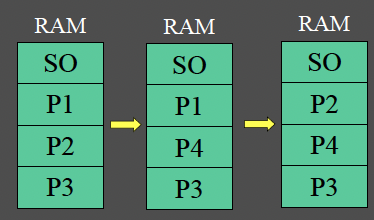
\includegraphics[width=0.5\linewidth]{images/table_swap.png}
\end{figure}
 
\begin{figure}[h]
    \centering
    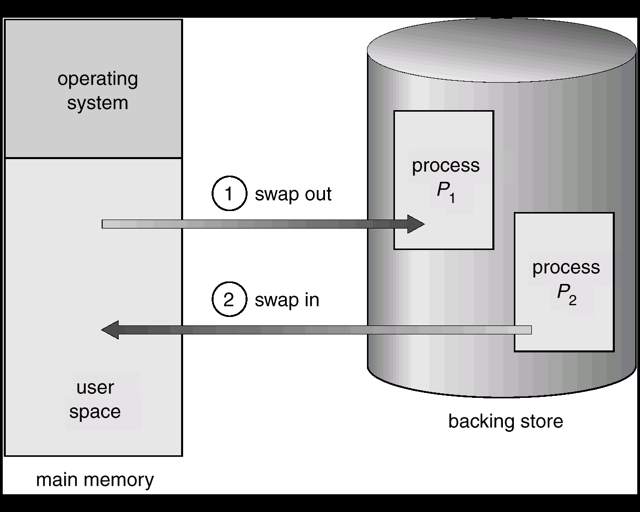
\includegraphics[width=0.5\linewidth]{images/swap-mem.png}
    \caption{Swap mem}
    \label{fig:swap-mem}
\end{figure}
Perché un programma possa essere \textbf{eseguito}, il suo codice deve trovarsi in \textbf{memoria} \textbf{primaria} (ma rivedremo questa affermazione quando parleremo della memoria virtuale)
Quindi, quando il SO riceve il \textbf{comando} di esecuzione di un programma, deve recuperare il codice del programma dalla memoria secondaria, e decidere in quale porzione della memoria primaria sistemarlo. ossia, a partire da quale indirizzo di RAM.

\section{Binding (associazione degli indirizzi)}
Un programma sorgente usa (tra l'altro) dati (variabili) e
istruzioni di controllo del flusso di computazione.
\begin{itemize}
    \item Quando il programma viene compilato e caricato in
    Memoria Primaria (MP) per essere eseguito, ad ogni
    variabile è associato l'\textbf{indirizzo} di una locazione di
    memoria che ne contiene il valore.
    \item Alle istruzioni di controllo del flusso di esecuzione del
    programma (ossia i salti condizionati e incondizionati) è
    associato l'indirizzo di destinazione del salto.
    \item L'operazione di associazione di variabili e istruzioni agli
    indirizzi di memoria è detta \textit{binding degli indirizzi}.
\end{itemize}

In altre parole, ad ogni variabile dichiarata nel programma viene fatto corrispondere l'indirizzo di una cella di memoria di RAM in cui verrà memorizzato il valore di quella variabile.
\begin{itemize}
    \item L'accesso alla variabile, in lettura e scrittura, corrisponde
    alla lettura e scrittura della cella di memoria il cui indirizzo
    è stato "legato" (con l'operazione di binding) alla variabile.
    \item Le istruzioni di salto, che permettono di implementare
    costrutti come \textit{if-then-else}, \textit{while}, ecc., sono associate agli
    indirizzi in RAM dove si trova l'istruzione con cui prosegue
    l'esecuzione del programma se il salto viene eseguito.
\end{itemize}

Ad esempio, un'istruzione C come:
\begin{verbatim}
counter = counter + 1;
\end{verbatim}
alla fine diventerà qualcosa del tipo:
\begin{verbatim}
load(R1, 10456)
Add(R1, #1);
store(R1, 10456)
\end{verbatim}
10456 è l'indirizzo della cella di memoria che contiene il
valore della variabile \textit{counter}. L'indirizzo 10456 è stato
associato alla variabile \textit{counter} durante la fase di binding
degli indirizzi.


Analogamente, un'istruzione C come:
\begin{verbatim}
while (counter <= 100) counter++;
\end{verbatim}
alla fine diventerà qualcosa del tipo:
\begin{verbatim}
100FC jgt(R1, #100, 10110) // jump if greater than
10100 load(R1, 10456)
10104 Add(R1, #1)
10108 store(R1, 10456)
1010C jmp(100FC)
10110 ... ...
\end{verbatim}

Rispetto all'indirizzo di istruzione del salto stesso, il \textit{while} della slide precedente potrebbe anche essere tradotto in assembler così:
\begin{verbatim}
100FC jgt(R1, #100, 00014) // jump if greater than
10100 load(R1, 10456)
10104 Add(R1, #1)
10108 store(R1, 10456)
1010C jmp(100FC)
10110 ... ...
\end{verbatim}

Perché un programma sorgente
possa essere eseguito deve passare
attraverso varie fasi. Il binding degli indirizzi avviene
in una di queste fasi:
\begin{itemize}
    \item compilazione
    \item caricamento (in RAM)
    \item esecuzione
\end{itemize}

\begin{figure}[h]
    \centering
    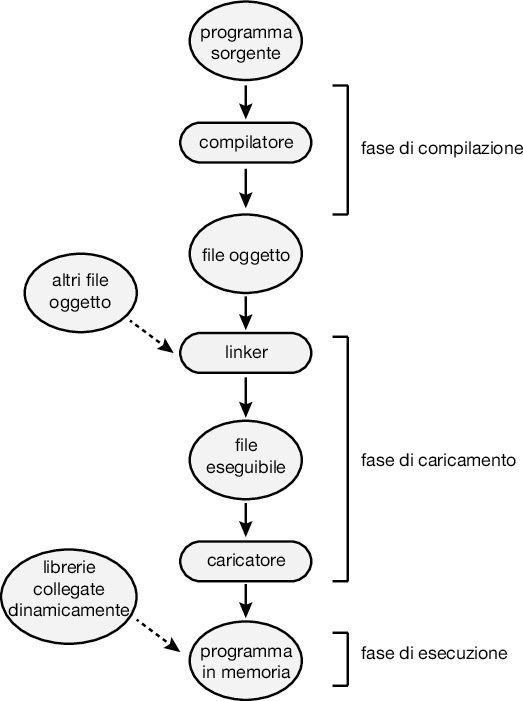
\includegraphics[width=0.25\linewidth]{images/process_compilation.png}
    \caption{Processo di compilazione da programma sorgente}
    \label{fig:compilate-process}
\end{figure}

\subsection{Quando?}
\begin{enumerate}
    \item In fase di Compilazione 
        \begin{itemize}
        \item viene generato codice assoluto o statico.
        \item Il compilatore deve conoscere l'indirizzo della cella di
        RAM a partire dal quale verrà caricato il programma,
        in modo da effettuare il \textit{binding} degli indirizzi
        (che avviene, appunto, in fase di compilazione).
        \item Se il SO deve scaricare temporaneamente il processo
        che usa quel codice in Memoria Secondaria (MS), come
        nell'esempio visto a inizio capitolo, quando lo ricarica
        in RAM deve rimetterlo esattamente dove si trovava
        prima. (Oppure?)
        \end{itemize}
    \item  In fase di caricamento in RAM
        \begin{itemize}
        \item Viene generato codice staticamente rilocabile.
        \item Il compilatore associa ad istruzioni e variabili degli
        indirizzi relativi rispetto all'inizio del programma,
        che inizia da un ipotetico indirizzo 0 virtuale.
        \item Gli indirizzi assoluti finali vengono generati in fase di
        caricamento del codice in Memoria Primaria (MP) in base all'indirizzo di
        MP a partire dal quale è caricato il codice.
        \item Il binding degli indirizzi, quindi, avviene in fase di
        caricamento del programma in RAM: se il processo che
        usa quel codice viene tolto dalla RAM, si può caricarlo
        in una posizione diversa solo rieffettuando la fase di
        caricamento (ma è più efficiente che ricompilare tutto).
        \end{itemize}
    \item In fase di esecuzione
        \begin{itemize}
        \item Viene generato codice dinamicamente rilocabile.
            \item Il codice in esecuzione usa sempre e solo indirizzi
            relativi.
            \item La trasformazione di un indirizzo relativo in uno
            assoluto viene fatta nell'istante in cui viene eseguita
            l'istruzione che usa quell'indirizzo.
            \item È necessario un opportuno supporto hardware per realizzare
            questo metodo senza perdita di efficienza.
            \item Si parla di \textit{binding dinamico} degli indirizzi.
            \item In opportuno registro di rilocazione viene usato per trasformare un indirizzo relativo nel corrispondente indirizzo assoluto durante l’esecuzione delle istruzioni.
            \item Il registro di rilocazione contiene l’indirizzo di partenza dell’area di RAM in cui è caricato il programma in esecuzione.
            \item La memory management Unit (MMU) si occuperà di trasformare gli indirizzi relativi in assoluti, usando il registro di rilocazione, per accedere alle celle di RAM indirizzate dalle istruzioni
            \item Lo spostamento del processo da un area all’altra della MP è realizzabile senza problema.
            \item Il SO deve solo ricordarsi dell’indirizzo della locazione di MP a partire dalla quale è memorizzato il processo
        \end{itemize}
        \nt{Per spostare i programmi da un’area di RAM ad un’altra ora basta cambiare l’indirizzo scritto nel registro di rilocazione (fig. 9.5 modificata)}
\end{enumerate}

\section{Spazio degli indirizzi (Logici e Fisici)}
Consideriamo codice dinamicamente rilocabile (d’ora in poi faremo sempre riferimento a codice dinamicamente rilocabile, se non indicato diversamente). Ogni indirizzo usato nel codice è riferito ad un ipotetico indirizzo 0 (zero): l’indirizzo della prima istruzione di cui è formato il codice.

Gli indirizzi utilizzati in un programma possono essere:
\begin{itemize}
    \item l'indirizzo di una cella di memoria che contiene una variabile
    \item l'indirizzo di un'istruzione di salto
\end{itemize}

Questi indirizzi rientrano nello \textbf{spazio di indirizzamento logico o virtuale}, che va da 0 all'ultima cella di memoria occupata. Quando il codice viene caricato in RAM, gli \textbf{indirizzi logici} generati dalla CPU vengono trasformati in \textbf{indirizzi fisici} attraverso il registro di rilocazione, permettendo di indirizzare correttamente la memoria fisica (RAM).

Lo \textbf{spazio di indirizzamento fisico} è l'insieme degli indirizzi fisici che dipende dall'area di memoria dove il sistema operativo ha caricato il programma.

Per i programmi con codice rilocabile dinamicamente esistono due tipi di indirizzi:
\begin{itemize}
    \item Indirizzi logici, che vanno da $0$ a $max$
    \item Indirizzi fisici, che vanno da $r+0$ a $r+max$, dove $r$ è l'indirizzo iniziale della RAM in cui il programma è caricato
\end{itemize}

Gli indirizzi logici vengono sempre mappati in indirizzi fisici per accedere correttamente alla RAM.

Le espressioni \textbf{spazio di indirizzamento logico} e \textbf{spazio di indirizzamento fisico} si riferiscono principalmente all'architettura di un sistema, non a singoli programmi.

Consideriamo un computer con un massimo di 64 Kbyte di RAM, ovvero 65536 byte. In questo contesto, possiamo dire che:
\begin{enumerate}
    \item Il computer può indirizzare $2^{16}$ byte di RAM.
    \item Gli indirizzi dei byte della RAM vanno da 0000 a FFFF in esadecimale (da 0 a $2^{16} - 1$).
    \item L'indirizzo di ciascun byte della RAM è rappresentato da 16 bit.
\end{enumerate}

Pertanto, lo \textbf{spazio di indirizzamento fisico} di questo computer è scritto su 16 bit e va da 0000 a FFFF, con una dimensione di 64 Kbyte.

Se un compilatore genera codice dinamicamente rilocabile e utilizza 12 bit (\textbf{perchè 12?}) per scrivere un indirizzo logico, lo \textbf{spazio di indirizzamento logico} di un programma sarà di massimo $2^{12}$ byte, ovvero 4 Kbyte. Nessun programma potrà superare questo limite, anche se può usare uno spazio logico inferiore.

Quindi, possiamo dire che lo spazio di indirizzamento logico dei programmi di questo computer è scritto su 12 bit, va da 0000 a 0FFF (esadecimale) ed è di 4 Kbyte.

In seguito, quando parleremo di spazi di indirizzamento, ci riferiremo a quelli dell'intera macchina, e non a quelli dei singoli programmi. Tuttavia, è possibile considerare un programma che occupa tutto lo spazio di indirizzamento logico della macchina.

\qs{}{Ha senso che la dimensione dello spazio di indirizzamento fisico sia diversa da quella dello spazio di indirizzamento logico in un sistema reale?}

In effetti, è comune che lo \textbf{spazio di indirizzamento fisico} e lo \textbf{spazio di indirizzamento virtuale} siano diversi. Nei processori moderni a 64 bit, lo spazio di indirizzamento fisico può variare da $2^{40}$ a $2^{64}$ byte (da 40 a 64 bit per gli indirizzi fisici). Tuttavia, non si usano sempre 64 bit per gli indirizzi fisici perché sono eccessivi, e un computer raramente ha una quantità di RAM pari al massimo indirizzabile dal processore (ad esempio, $2^{40}$ byte = 1 Terabyte = 1000 Gigabyte).

Sistemi operativi e applicazioni adottano spazi di indirizzamento virtuali che variano tipicamente da $2^{48}$ a $2^{64}$ byte, ovvero da 48 a 64 bit per gli indirizzi virtuali.

In generale, per i computer moderni vale la relazione:
\[
|\text{RAM}| \neq |\text{spazio di indirizzamento fisico}| \neq |\text{spazio di indirizzamento virtuale}|
\]
E di solito:
\[
|\text{RAM}| < |\text{spazio di indirizzamento fisico}| < |\text{spazio di indirizzamento virtuale}|
\]

In molti casi, per vincoli architetturali e dimensionali, la quantità effettiva di RAM di un computer è molto inferiore allo spazio di indirizzamento fisico. Pertanto, è spesso vero che:
\[
|\text{RAM}|_{\text{effettiva}} \leq |\text{RAM}|_{\text{massima}} \ll |\text{spazio fisico}| < |\text{spazio virtuale}|
\]
\clm{}{}{
Ad esempio, nei processori Intel Core i7 lo spazio di indirizzamento fisico è scritto su 52 bit, mentre quello virtuale è su 48 bit, quindi può capitare che:
\[
|\text{spazio fisico}| > |\text{spazio virtuale}|
\]
}

\qs{}{
Se un sistema ha uno spazio di indirizzamento virtuale di $X$ byte, significa che possiamo scrivere un programma che occupa al massimo $X$ byte, cioè usa indirizzi virtuali da 0 a $X-1$. Tuttavia, un programma può girare su una macchina in cui:
\[
|\text{RAM}| < |\text{spazio fisico}| < X?
\]
}

Questo aspetto sarà approfondito nel capitolo sulla \textbf{memoria virtuale}.


\section{Le librerie}
\dfn{}{
Una \textbf{libreria} è una collezione di subroutine di uso comune messe a disposizione dei programmatori per lo sviluppo software. Ad esempio, la libreria matematica del C fornisce funzioni come \texttt{sqrt(x)} per calcolare la radice quadrata.}

Le librerie sono utili perché permettono di riutilizzare codice già esistente, evitando ai programmatori di doverlo riscrivere ogni volta. Sebbene "libreria" sia una traduzione impropria di "library", il termine è ormai comunemente accettato.

\subsection{Tipi di Librerie}

Esistono principalmente due tipi di librerie:

\begin{enumerate}
    \item \textbf{Librerie statiche}: le subroutine sono collegate al programma principale durante la fase di compilazione o di caricamento, diventando parte dell'eseguibile. Tuttavia, ciò può portare a duplicazione di codice, sia su disco che in RAM, soprattutto se più programmi usano la stessa libreria. Inoltre, il codice di una libreria statica viene caricato in RAM anche se non viene utilizzato durante l'esecuzione del programma.

    \item \textbf{Librerie dinamiche}: vengono caricate in RAM solo al momento in cui il programma chiama una subroutine specifica, ossia a \textbf{run-time}. Il programma specifica solo il nome della subroutine, e il sistema operativo carica la libreria nello spazio di memoria assegnato al processo. Queste librerie sono anche dette \textbf{librerie condivise}, perché possono essere utilizzate da più processi contemporaneamente, evitando la duplicazione di codice in RAM. Inoltre, le versioni aggiornate delle librerie dinamiche possono sostituire le vecchie senza dover ricompilare i programmi che le utilizzano.
\end{enumerate}

\subsection{Estensioni delle Librerie Dinamiche}

In Unix, Linux e Solaris, le librerie dinamiche hanno estensione \texttt{.so} (shared object) e si trovano solitamente nella directory \texttt{/lib}. In ambiente Windows, le librerie dinamiche hanno estensione \texttt{.DLL} (Dynamic Link Library) e si trovano nella cartella \texttt{C:\textbackslash WINDOWS\textbackslash system32}.

\section{Tecniche di gestione della memoria primaria}
Le principali tecniche di gestione della \textbf{Memoria Principale (MP)} vanno dalle più semplici alle più complesse. Alcune di queste tecniche sono ormai obsolete, ma aiutano a comprendere concetti più avanzati. Le tecniche includono:

\begin{itemize}
    \item \textbf{Swapping}
    \item \textbf{Allocazione contigua a partizioni multiple fisse}
    \item \textbf{Allocazione contigua a partizioni multiple variabili}
    \item \textbf{Paginazione}
    \item \textbf{Paginazione a più livelli}
\end{itemize}

\subsection*{Swapping}

\dfn{}{Lo \textbf{swapping} consiste nel salvare in memoria secondaria (hard disk) l'immagine di un processo non in esecuzione (\textit{swap out}) e ricaricarla in MP (\textit{swap in}) prima di assegnarle la CPU.}

Questa tecnica permette di attivare più processi di quanti la sola MP possa contenere, utilizzando un'area dell'hard disk chiamata \textbf{area di swap}, riservata al sistema operativo. Tuttavia, se il processo viene ricaricato in una diversa area di MP, è necessario utilizzare codice dinamicamente rilocabile.

\subsubsection*{Problemi dello Swapping}

Il principale problema dello swapping è il tempo impiegato per copiare il codice e i dati di un processo tra l'hard disk e la RAM, che è nell'ordine dei millisecondi. Poiché in un millisecondo un singolo core di una moderna CPU può eseguire milioni di istruzioni, l'overhead di tempo risultante dallo swapping è generalmente considerato inaccettabile.

Di conseguenza, lo \textbf{swapping di interi processi} è ormai caduto in disuso nei moderni sistemi operativi, salvo rare eccezioni.

\subsubsection*{L'Idea di Fondo dello Swapping}

Nonostante l'obsolescenza dello swapping, l'idea di fondo rimane valida: utilizzare parte della memoria secondaria per estendere la memoria primaria, permettendo l'esecuzione di un numero maggiore di processi rispetto a quanto potrebbe ospitare la sola RAM. Questa idea sarà ripresa nel capitolo sulla \textbf{memoria virtuale}.


\section{Allocazione contigua della Memoria Primaria}
In un computer, la \textbf{Memoria Principale (MP)} è solitamente divisa in due partizioni:
\begin{itemize}
    \item una per il \textbf{Sistema Operativo (SO)}
    \item una per i \textbf{processi utente}.
\end{itemize}

Il sistema operativo si posiziona nella stessa area di memoria puntata dal \textbf{vettore delle interruzioni}, che è spesso allocato nella parte bassa della memoria.

\subsection*{Protezione della memoria}

Nei sistemi operativi più semplici (ad esempio MS-DOS), l'area non assegnata al SO viene occupata da un solo processo. La protezione della MP consiste nella protezione delle aree di memoria del SO.

\subsubsection*{Registro Limite e Registro di Rilocazione}

Il \textbf{registro limite} è inizializzato dal SO e garantisce che ogni indirizzo logico usato dal processo utente sia inferiore al valore scritto nel registro. Poiché si utilizza codice dinamicamente rilocabile, il \textbf{registro di rilocazione} viene usato per trasformare l'indirizzo logico in indirizzo fisico.

\begin{itemize}
    \item \textbf{Registro di rilocazione}: 100.040
    \item \textbf{Registro limite}: 74.600
\end{itemize}

Gli indirizzi fisici validi vanno da 100.040 a 174.640 (vedi Fig. \ref{fig:9.6}).
\begin{figure}[h]
    \centering
    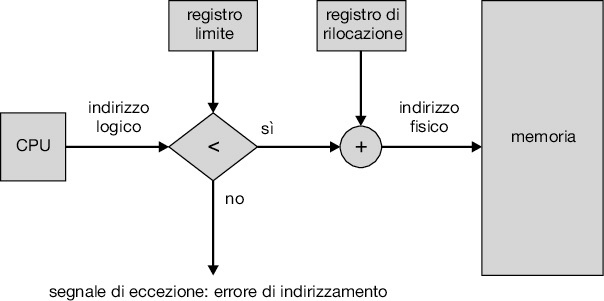
\includegraphics[width=0.5\linewidth]{images/protez_meme.png}
    \caption{Protezione memoria}
    \label{fig:9.6}
\end{figure}

\subsection{Allocazione a partizioni multiple fisse}
Nell'allocazione a partizioni fisse:
\begin{itemize}
    \item La memoria è divisa in \textbf{partizioni di dimensione fissa}, che non devono necessariamente essere tutte uguali.
    \item Ogni partizione contiene un \textbf{unico processo} dall'inizio alla fine della sua esecuzione.
    \item Il \textbf{grado di multiprogrammazione} è determinato dal numero di partizioni.
    \item Quando un processo termina, la partizione può essere occupata da un altro processo.
\end{itemize}

Il meccanismo di \textbf{registri limite e di rilocazione} protegge le partizioni da accessi non autorizzati. Durante il \textit{context switch}, il \textbf{dispatcher} carica:
\begin{itemize}
    \item Nel registro di rilocazione, l'indirizzo di partenza della partizione assegnata al processo.
    \item Nel registro limite, la dimensione della partizione.
\end{itemize}

Questa tecnica, utilizzata nel \textbf{IBM OS/360}, richiede CPU dotate di registri di rilocazione e limite, ma non è più utilizzata nei sistemi operativi moderni per i seguenti svantaggi:
\begin{itemize}
    \item Il grado di multiprogrammazione è limitato dal numero di partizioni disponibili.
    \item Si verifica \textbf{frammentazione interna}, dove una parte della partizione rimane inutilizzata se il processo è più piccolo della partizione stessa.
    \item Si può verificare \textbf{frammentazione esterna}, quando lo spazio libero disponibile è frammentato in più aree non contigue e quindi non utilizzabile per un nuovo processo di dimensione maggiore.
    \item L'arrivo di un processo più grande della partizione più grande non può essere gestito.
\end{itemize}

\textbf{Frammentazione interna}:
\begin{itemize}
    \item Parte dello spazio di memoria di una partizione viene sprecato se il processo è più piccolo della partizione stessa.
\end{itemize}

\textbf{Frammentazione esterna}:
\begin{itemize}
    \item Se la memoria libera è frammentata in più blocchi non contigui, pur avendo spazio sufficiente in totale, non può essere utilizzata per allocare nuovi processi.
\end{itemize}

L’allocazione a partizioni fisse ha anche altri problemi:
\qs{}{Che succede se arriva un processo più grande della partizione più grande?}
\clm{}{}{Notate che se si aumenta la dimensione media delle partizioni, aumenta anche la frammentazione interna, e diminuisce il grado di multiprogrammazione}

\section{Allocazione a partizioni multipli variabili}
Nell'allocazione a partizioni variabili:
\begin{itemize}
    \item Ogni processo riceve una quantità di memoria esattamente pari alla sua dimensione.
    \item Quando un processo termina, lascia un "buco" in RAM che può essere occupato da un altro processo.
    \item Tuttavia, nel tempo si creano \textbf{buchi sparsi e più piccoli}, rendendo difficile l'allocazione di nuovi processi.
\end{itemize}

\begin{figure}[h]
    \centering
    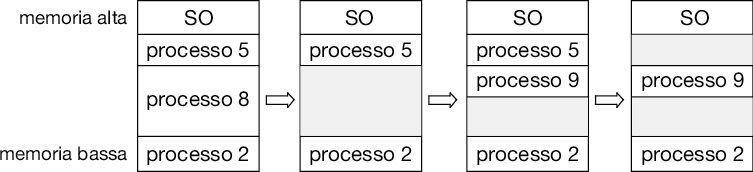
\includegraphics[width=0.5\linewidth]{images/ram_buchi.png}
    \caption{Buchi Ram}
    \label{fig:ram_hole}
\end{figure}
Il sistema operativo (SO) deve:
\begin{itemize}
    \item Tenere traccia delle aree di memoria libere e occupate.
    \item Aggiornare continuamente le informazioni quando un processo nasce o termina.
    \item Assegnare una partizione sufficientemente grande quando un nuovo processo deve essere caricato.
\end{itemize}

\subsection*{Strategie di Allocazione}
Esistono diverse strategie per scegliere quale partizione assegnare a un processo:
\begin{itemize}
    \item \textbf{First Fit}: seleziona la prima partizione abbastanza grande da ospitare il processo.
    \item \textbf{Best Fit}: seleziona la partizione più piccola che può contenere il processo.
    \item \textbf{Worst Fit}: seleziona la partizione più grande disponibile.
\end{itemize}

\textbf{Osservazioni sperimentali}:
\begin{itemize}
    \item La strategia \textbf{Worst Fit} tende a funzionare peggio in termini di utilizzo della memoria, poiché lascia spazi grandi frammentati.
    \item Le strategie \textbf{Best Fit} e \textbf{First Fit} hanno prestazioni simili, ma si preferisce \textbf{First Fit} poiché è più veloce, dato che interrompe la ricerca al primo spazio sufficiente.
\end{itemize}

\subsection{La frammentazione}
Nel tempo, l'allocazione a partizioni variabili può portare alla formazione di piccoli \textbf{buchi non contigui} in RAM:
\begin{itemize}
    \item Circa \textbf{1/3 a 1/2 della memoria principale} (MP) può essere sprecato a causa della \textbf{frammentazione esterna}, ossia la presenza di buchi di memoria troppo piccoli per ospitare un processo.
    \item Esiste anche il problema della \textbf{frammentazione interna}, dovuto all'impossibilità di tenere traccia di buchi molto piccoli che vengono quindi aggregati a partizioni adiacenti, causando uno \textbf{spreco nascosto}.
\end{itemize}

\subsubsection*{Compattazione della Memoria}

Una tecnica per recuperare la memoria inutilizzata è la \textbf{compattazione}:
\begin{itemize}
    \item Spostare le partizioni occupate dai processi in modo che siano tutte \textbf{contigue}, liberando un unico grande buco libero.
    \item La compattazione richiede la \textbf{rilocazione dinamica} del codice e dei dati dei processi.
    \item Questo processo è \textbf{costoso in termini di tempo} e durante la compattazione il sistema non è utilizzabile.
\end{itemize}

\section{Paginazione della memoria}
\dfn{}{
L’allocazione contigua della memoria principale presenta quindi diversi problemi.
L’alternativa è ammettere che l’area di memoria allocata ad un processo possa essere in realtà suddivisa in tanti pezzi non contigui fra loro
Se tutti i “pezzi” hanno la stessa dimensione allora il termine esatto per indicare questa tecnica è: paginazione della memoria (primaria)}

\subsection{Metodo di base}
La \textbf{Memoria Primaria} (o lo \textbf{spazio di indirizzamento fisico}) è suddivisa in unità dette \textbf{frame} (o pagine fisiche), con le seguenti caratteristiche:
\begin{itemize}
    \item I \textbf{frame} sono tutti della stessa dimensione, che è sempre una \textbf{potenza di due} (ad esempio: 512, 1024, 2048, fino a 8192 byte).
    \item Lo spazio di indirizzamento fisico del processo è visto come un \textbf{unico spazio contiguo} di indirizzi, ma nella realtà è suddiviso in \textbf{pagine logiche}, ciascuna di dimensione uguale ai frame fisici.
\end{itemize}

Per eseguire un processo con \textbf{x pagine}:
\begin{itemize}
    \item Il Sistema Operativo (\textbf{SO}) cerca \textbf{x frame} liberi in cui caricare le pagine del processo. Questi frame non devono essere adiacenti e le pagine possono essere caricate in un ordine qualsiasi.
    \item Ogni processo ha una propria \textbf{Tabella delle Pagine} (o \textbf{Page Table}, \textbf{PT}): un array le cui \emph{entry} contengono i numeri dei frame in cui le pagine del processo sono state caricate.
    \item Il SO tiene traccia dei \textbf{frame liberi} nella memoria primaria, utilizzandoli per memorizzare le pagine di nuovi processi.
\end{itemize}

\subsection*{Struttura della Tabella delle Pagine}
\begin{itemize}
    \item Ogni \emph{entry} della Page Table rappresenta una pagina del processo.
    \item L'indice di ciascuna entry corrisponde al numero della pagina, mentre il valore dell'entry contiene il numero del frame dove è stata memorizzata la pagina.
\end{itemize}
% \begin{figure}[h] \centering 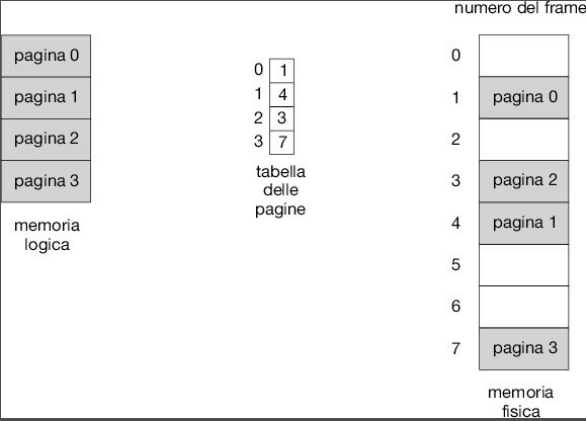
\includegraphics[width=0.50\linewidth]{images/structure_table_pagination.png} \caption{Table Pagination} \label{fig:9.9} \end{figure}
\subsection*{Problema degli Indirizzi Virtuali}
Gli \textbf{indirizzi relativi (o virtuali)} del programma, una volta caricati in RAM, non funzionano più come indirizzi lineari contigui. Ad esempio:
\begin{itemize}
    \item Un'istruzione come \texttt{jmp\_if\_odd R1,C} deve saltare a un indirizzo specifico (ad es. 0004), ma in RAM non esiste più un punto lineare di partenza.
    \item La soluzione è \textbf{riconsiderare} gli indirizzi virtuali, non più come indirizzi lineari, ma come indirizzi all'interno della Page Table, utilizzando \textbf{conversioni da indirizzi logici a indirizzi fisici}.
\end{itemize}


Indirizzi Logici e Fisici, vedere registrazione 25/10/2024 min Circa 30

\subsubsection{Paginazione: metodo di base}
Gli indirizzi logici diventano delle coppie di valori, in cui:
\begin{itemize}
    \item il primo elemento della coppia specifica il numero della pagina all’interno della quale si trova la cella di memoria che vogliamo indirizzare;
    \item il secondo elemento specifica la posizione (o offset) della cella di memoria che vogliamo indirizzare rispetto ad un ipotetico indirizzo 0 (zero), ovvero l’indirizzo del primo byte della pagina specificata dal primo elemento della coppia.
\end{itemize}
Quindi un indirizzo logico assume la forma: $(\text{pagina}, \text{offset})$.

\nt{
    Come vedremo più avanti, sotto opportune condizioni gli indirizzi logici lineari e gli indirizzi logici specificati come coppie di valori coincidono.
}

Un indirizzo logico viene tradotto in uno fisico secondo il seguente processo:
\begin{itemize}
    \item Il numero di pagina $p$ viene usato come indice nella \textit{page table} del processo per individuare il frame $f$ in cui è contenuta la pagina.
    \item Una volta noto il frame $f$ che contiene la pagina $p$, l’offset $d$ (dove "d" sta per \textit{displacement}) può essere applicato a partire dall’inizio del frame per indirizzare il byte specificato dalla coppia $(p, d)$.
\end{itemize}

Vediamo più in dettaglio: ogni informazione all’interno del computer, incluso un indirizzo logico, è in definitiva una sequenza di bit. Ad esempio: 001100010101.

Abbiamo deciso di dividere un indirizzo logico in due parti. Se abbiamo a disposizione 12 bit in tutto, dobbiamo scegliere quanti usare per specificare il numero della pagina e quanti per l’offset all’interno della pagina.

Ad esempio, possiamo decidere di utilizzare 4 bit per rappresentare il numero della pagina e i restanti 8 bit per l’offset. In questo caso, l’indirizzo logico 001100010101 rappresenta:
\begin{itemize}
    \item pagina: 3
    \item offset: 21
\end{itemize}

La scelta del numero di bit da utilizzare per scrivere il numero di pagina e l’offset dipende dall’hardware su cui dovrà girare il sistema operativo, il quale impone:
\begin{itemize}
    \item il numero di bit su cui va scritto un indirizzo logico (ad esempio $m$ bit);
    \item la dimensione di un frame, e quindi di una pagina (ad esempio $2^n$ byte).
\end{itemize}

Di conseguenza, dobbiamo utilizzare $n$ bit per rappresentare l'offset all'interno di una pagina/frame, e il numero di bit usati per rappresentare il numero di pagina sarà pari a $m - n$ bit.

\nt{
    A questo punto, la dimensione dello spazio di indirizzamento logico è stabilita come $2^{(m-n)} \times 2^n$ byte.
}

\ex{Esempio di Spazio di Indirizzamento Logico}{
    Consideriamo una macchina in cui i frame hanno dimensione $2^{12}$ byte, ovvero 4096 byte. Di conseguenza, anche la dimensione di una pagina nello spazio di indirizzamento logico del sistema sarà di 4096 byte (quindi $n = 12$).
    
    Se la macchina mette a disposizione $m = 22$ bit per rappresentare un indirizzo logico, allora il numero di bit necessari per il numero di pagina sarà $m - n = 10$ bit.
    
    In questo caso, lo spazio di indirizzamento logico della macchina risulterà pari a:
    \[
    (2^{10} \text{ pagine}) \times (2^{12} \text{ byte}) = 4 \text{ megabyte}
    \]
}

\begin{center}
    \textbf{Struttura di un Indirizzo Logico}
\end{center}
\begin{itemize}
    \item \textbf{Numero di Pagina (p)}: $m - n$ bit
    \item \textbf{Offset di Pagina (d)}: $n$ bit
\end{itemize}

\nt{
    Qui possiamo osservare uno dei tanti casi di interazione tra il sistema operativo e l’hardware sottostante. È infatti l’hardware a decidere la dimensione dei frame e il numero di bit su cui rappresentare un indirizzo logico. Il sistema operativo, quindi, deve adeguarsi a queste impostazioni.
    
    Questa configurazione consente una traduzione efficiente degli indirizzi logici in indirizzi fisici direttamente a livello hardware. Alcune parti di un sistema operativo sono infatti progettate in base allo specifico hardware su cui girerà il sistema, al fine di sfruttare al meglio le caratteristiche hardware e minimizzare l’overhead introdotto.
}

\clm{Scelta della Dimensione dei Frame}{}{
    Nei processori moderni, è possibile scegliere tra vari valori per la dimensione dei frame, e questa scelta, una volta effettuata, rimane fissa. Ad esempio:
    \begin{itemize}
        \item I processori ARM, utilizzati negli iPhone e negli iPad, permettono di scegliere tra 4KB, 16KB, 64KB, 1MB e 16MB come dimensione di un frame.
        \item La famiglia dei processori Intel, dal Pentium fino ai Core i9, consente di scegliere tra 4KB e 4MB.
        \item Gli Intel Itanium-2 offrono una gamma più ampia, con opzioni tra 4KB, 8KB, 64KB, 256KB, 1MB, 4MB, 16MB e 256MB.
    \end{itemize}
}

\dfn{Traduzione degli Indirizzi Logici in Indirizzi Fisici}{
    Definiamo più precisamente l'operazione di traduzione da indirizzi logici a indirizzi fisici. Un indirizzo logico è formato da due componenti $(p, d)$:
    \begin{itemize}
        \item \textbf{Numero di Pagina (p)}: utilizzato come indice per selezionare la entry corrispondente nella \textit{Page Table}, che contiene il numero del frame in cui è caricata la pagina.
        \item \textbf{Offset di Pagina (d)}: utilizzato all’interno del frame individuato al passo precedente per localizzare il byte specificato dall’indirizzo logico.
    \end{itemize}
}

\subsubsection{Paginazione: traduzione degli indirizzi}
Possiamo ora riassumere e integrare quanto detto finora, osservando che:

\begin{enumerate}
    \item Gli indirizzi logici nello spazio di indirizzamento logico possono essere interpretati come valori lineari oppure come coppie $(\text{pagina}, \text{offset})$.
    \item Ciascuna entry di una tabella delle pagine può contenere il numero del frame o, alternativamente, l’indirizzo di partenza del frame. Tuttavia, per ragioni pratiche, viene scelta la prima opzione: memorizzare il numero del frame.
\end{enumerate}

\nt{
    Ecco quindi la doppia natura degli indirizzi logici, che sono contemporaneamente valori lineari e coppie $(\text{pagina}, \text{offset})$.
}

Consideriamo uno spazio di indirizzamento logico di dimensione $2^m$ byte, e assumiamo che ogni pagina abbia una dimensione pari a $2^n$ byte. Un indirizzo logico lineare scritto su $m$ bit può quindi essere scomposto in:
\begin{itemize}
    \item i bit più significativi $(m - n)$, che indicano il numero di pagina $p$;
    \item i bit meno significativi $n$, che rappresentano l’offset $d$.
\end{itemize}

\begin{center}
    \textbf{Struttura di un Indirizzo Logico}
\end{center}
\begin{itemize}
    \item \textbf{Numero di Pagina (p)}: $(m - n)$ bit
    \item \textbf{Offset di Pagina (d)}: $n$ bit
\end{itemize}

\ex{Esempio di Spazio di Indirizzamento Logico}{
    Supponiamo di avere uno spazio di indirizzamento logico di 16 byte, quindi gli indirizzi logici sono rappresentati con $m = 4$ bit, poiché $2^4 = 16$. Ogni pagina ha dimensione $2^2 = 4$ byte, con $n = 2$.

    Di conseguenza, gli indirizzi logici vanno da $0000$ a $1111$, mentre il programma che occupa questo spazio è costituito dalle istruzioni/dati etichettati come "a, b, c, d, e, f, g, h, i, l, m, n" che coprono tre pagine, dove ciascuna istruzione/dato occupa un byte.
    
    \nt{
        In questo esempio, lo spazio di indirizzamento logico del programma è suddiviso in pagine. Gli indirizzi di istruzioni e dati, che costituiscono lo spazio di indirizzamento logico, sono quindi valori consecutivi che vanno da $0000$ (prima istruzione) a $1011$ (ultima istruzione).
    }
    
    Osserviamo come gli $(m - n)$ bit più significativi di ciascun indirizzo rappresentano il numero di pagina, mentre i restanti $n$ bit meno significativi indicano l'offset all'interno della pagina.
}

\begin{center}
    \begin{tabular}{cc}
        \textbf{Indirizzo Logico} & \textbf{Contenuto} \\
        \hline
        \textbf{00 00} & a \\
        \textbf{00 01} & b \\
        \textbf{00 10} & c \\
        \textbf{00 11} & d \\
        \textbf{01 00} & e \\
        \textbf{01 01} & f \\
        \textbf{01 10} & g \\
        \textbf{01 11} & h \\
        \textbf{10 00} & i \\
        \textbf{10 01} & l \\
        \textbf{10 10} & m \\
        \textbf{10 11} & n \\
    \end{tabular}
\end{center}

Ogni indirizzo è quindi composto da:
\begin{itemize}
    \item I primi due bit, che rappresentano il numero di pagina:
    \begin{itemize}
        \item $00$ per la pagina 0
        \item $01$ per la pagina 1
        \item $10$ per la pagina 2
    \end{itemize}
    \item Gli ultimi due bit, che rappresentano l’offset all’interno della pagina.
\end{itemize}

\nt{
    Supponiamo ora di caricare il programma in RAM. Utilizziamo 5 bit per rappresentare un indirizzo fisico, quindi lo spazio di indirizzamento fisico ha dimensione pari a $2^5 = 32$ byte. Tuttavia, la nostra macchina è dotata di soli 20 byte di RAM, suddivisi in 5 frame, ciascuno con un indirizzo che va da $00000$ a $10011$.
}

\ex{Esempio di Traduzione Indirizzo Logico in Indirizzo Fisico}{
    Consideriamo l’indirizzo logico $0010$. La sua conversione in un indirizzo fisico procede così:
    \begin{enumerate}
        \item \textbf{Numero di Pagina}: il numero di pagina (0) è utilizzato per accedere alla \textit{Page Table}, che ci indica che la pagina 0 è caricata nel frame 4.
        \item \textbf{Offset}: l'offset di 2 bit $(10)$ viene applicato a partire dall’indirizzo iniziale del frame 4.
    \end{enumerate}
    Di conseguenza, l’indirizzo fisico risultante è $10010$.
}

% \begin{figure}[h] \centering 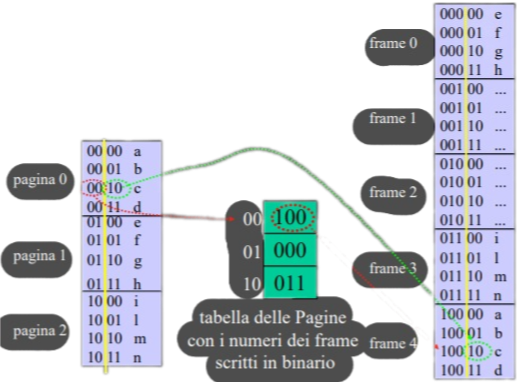
\includegraphics[width=0.25\linewidth]{images/pagination_example.png} \caption{Esempo di paginazione} \label{fig:9.10} \end{figure}

\clm{Struttura di un Indirizzo Fisico}{}{
    Notiamo un aspetto importante: nei nostri indirizzi fisici, i bit più significativi (5 - 2 = 3 bit) indicano il numero di frame corrispondente. Ad esempio, per l’indirizzo $10010$, i primi 3 bit $100$ identificano il frame 4.
}

\nt{
    Le pagine e i frame sono configurati per avere una dimensione $|P|$ pari a una potenza di 2, ossia $|P| = 2^n$. Grazie a questa proprietà, l'offset all'interno di ogni pagina o frame varia da una configurazione di tutti zeri a una di tutti uno:
    \[
        \text{Offset valido: } 00 \dots 00 \text{ a } 11 \dots 11.
    \]
    Di conseguenza, l’indirizzo di partenza di ogni pagina o frame richiede che gli $n$ bit meno significativi siano impostati a 0.
}

\clm{Struttura degli Indirizzi di Partenza}{}{
    Gli indirizzi logici di inizio pagina nello spazio di indirizzamento di un programma avranno la forma seguente:
    \[
        \begin{array}{l}
            00 \dots 00 \; 00 \dots 00 \quad \text{inizio della pagina 0} \\
            00 \dots 01 \; 00 \dots 00 \quad \text{inizio della pagina 1} \\
            00 \dots 10 \; 00 \dots 00 \quad \text{inizio della pagina 2} \\
            00 \dots 11 \; 00 \dots 00 \quad \text{inizio della pagina 3}
        \end{array}
    \]
    Lo stesso vale per i frame nello spazio di indirizzamento fisico.
}

\nt{
    Se rimuoviamo gli $n$ bit meno significativi da un indirizzo logico di $m$ bit, i rimanenti $m - n$ bit contano semplicemente le pagine (in binario) in cui è suddiviso lo spazio di indirizzamento logico. Ad esempio:
    \[
        \begin{array}{l}
            00 \dots 00 = \text{pagina 0} \\
            00 \dots 01 = \text{pagina 1} \\
            00 \dots 10 = \text{pagina 2} \\
            00 \dots 11 = \text{pagina 3}
        \end{array}
    \]
    Questa logica vale anche per i frame nello spazio fisico, utilizzando un numero di bit adeguato per rappresentare i frame.
}

\ex{Ricostruzione dell'Indirizzo Fisico}{
    Supponiamo di avere un indirizzo logico in cui il numero di pagina e l’offset sono rappresentati come segue:
    \[
        \text{Numero di pagina } = 001010, \quad \text{Frame } = 1110001
    \]
    \[
        \text{Offset } = 101010
    \]
    Allora, l’indirizzo logico diventa $001010101010$, mentre l’indirizzo fisico corrispondente sarà $1110001101010$.
}

\nt{
    La conversione da indirizzo logico a fisico si basa sull’operazione di somma dell'indirizzo base del frame con l'offset, ad esempio:
    \[
        \begin{array}{l}
            \text{Indirizzo base del frame: } 1110001000000 \\
            \text{Offset: } \phantom{\text{Indirizzo base del frame: }} 101010
        \end{array}
    \]
    Somma:
    \[
        1110001000000 + 101010 = 1110001101010
    \]
}

\clm{Efficienza della Traduzione}{}{
    Se le dimensioni di pagine e frame sono potenze di due:
    \begin{enumerate}
        \item Non è necessario effettuare la somma tra l'indirizzo base del frame e l'offset, risparmiando tempo di calcolo.
        \item Non è necessario memorizzare l'indirizzo di base in ogni entry della page table, ma solo il numero del frame, poiché gli $n$ bit meno significativi dell'indirizzo di partenza sono tutti a 0, con un risparmio di spazio.
    \end{enumerate}
    Generare un indirizzo fisico diventa quindi un’operazione di concatenazione veloce tra il numero di frame e l'offset, eseguibile direttamente dall’hardware.
}

\nt{
    Quando le dimensioni di pagine e frame sono potenze di due, possiamo interpretare l’operazione di calcolo dell'indirizzo fisico come una concatenazione, anziché una somma:
    \[
        1110001000000 + 101010 = 1110001101010 \quad \Rightarrow \quad 1110001 \text{ “attaccato a” } 101010.
    \]
    Usando potenze di due, la costruzione dell'indirizzo fisico è più semplice e può essere gestita velocemente dall’hardware.
}

\ex{Esempio: Dimensione della Page Table}{
    Consideriamo un sistema in cui:
    \begin{itemize}
        \item l’indirizzo fisico è su 38 bit,
        \item l’indirizzo logico è su 40 bit,
        \item una pagina è di 8 Kbyte, quindi $2^{13}$ byte.
    \end{itemize}
    
    La dimensione della page table più grande possibile per questo sistema si calcola come segue:
    
    \begin{enumerate}
        \item \textbf{Calcolo del numero di entry nella page table}:
        \[
            \frac{2^{40} \text{ byte}}{2^{13} \text{ byte}} = 2^{27} \text{ entry}.
        \]
        
        \item \textbf{Numero di bit necessari per ogni entry}: Ogni entry deve essere in grado di indirizzare un frame nello spazio fisico. Lo spazio di indirizzamento fisico è diviso in:
        \[
            \frac{2^{38} \text{ byte}}{2^{13} \text{ byte}} = 2^{25} \text{ frame}.
        \]
        Il numero minimo di byte per rappresentare un frame è di 4 byte.
        
        \item \textbf{Calcolo della dimensione totale della page table}:
        \[
            2^{27} \times 2^2 \text{ byte} = 2^{29} \text{ byte} = 512 \text{ Mbyte}.
        \]
    \end{enumerate}
}
La paginazione permette di separare lo spazio di indirizzamento logico da quello fisico. Ogni programma “vede” la memoria come uno spazio contiguo che parte sempre dall'indirizzo logico 0, ma in realtà il programma è distribuito in diversi frame fisici, sparsi in memoria assieme ad altri programmi.
La paginazione introduce una protezione automatica dello spazio di indirizzamento. Un processo può accedere solo ai frame elencati nella sua page table, poiché ogni page table viene gestita e costruita dal sistema operativo per ciascun processo.

\clm{Vantaggi e Limiti della Paginazione}{}{
    \begin{itemize}
        \item \textbf{Eliminazione della frammentazione esterna}: Ogni frame libero può essere utilizzato per memorizzare una pagina, riducendo gli sprechi di memoria.
        \item \textbf{Frammentazione interna}: Rimane una media di mezza pagina per processo, poiché l’ultima pagina del processo può non occupare completamente il frame assegnato.
        \item \textbf{Rilocazione dinamica}: La paginazione implementa una forma di rilocazione dinamica, dove ogni pagina è mappata su un diverso valore del registro di rilocazione, ossia l’indirizzo di partenza del frame che contiene la pagina.
    \end{itemize}
}

\subsection{Rilocazione Dinamica}

\subsubsection{Rilocazione Dinamica Tramite Registri di Limite e di Rilocazione}
La \textbf{rilocazione dinamica} viene gestita inizialmente utilizzando due registri principali:
\begin{itemize}
    \item \textbf{Registro di limite}: Controlla che l’indirizzo logico rientri nello spazio di indirizzamento del processo. Se l’indirizzo eccede questo limite, il sistema lancia un’eccezione di indirizzamento.
    \item \textbf{Registro di rilocazione}: Viene usato per traslare l’indirizzo logico approvato in un indirizzo fisico, aggiungendo il valore del registro di rilocazione all’indirizzo logico (vedi Fig. 9.6).
\end{itemize}
Questo approccio verifica dunque prima la validità dell'indirizzo logico rispetto allo spazio di indirizzamento del processo, per poi calcolare l’indirizzo fisico finale.
\subsubsection{Rilocazione Dinamica di Ogni Singola Pagina Tramite la Page Table}
Con la \textbf{paginazione}, la gestione della rilocazione dinamica cambia in quanto:
\begin{itemize}
    \item La suddivisione in pagine elimina la necessità di un controllo tramite il registro limite. 
    \item Ogni indirizzo logico è diviso in \textbf{numero di pagina} e \textbf{offset}, dove l’offset rappresenta sempre una posizione interna al frame associato, eliminando il rischio di indirizzamenti fuori dai limiti (vedi Fig. 9.8).
\end{itemize}
In questo caso, il controllo e la mappatura degli indirizzi sono effettuati dalla page table, la quale memorizza l’indirizzo di ciascun frame per ogni pagina del processo attivo.

\subsection{Dimensione delle Pagine e Gestione della Tabella delle Pagine}

\subsubsection{Dimensione Storica delle Pagine}
Nel tempo, la \textbf{dimensione delle pagine} di memoria è aumentata progressivamente per adattarsi alle esigenze di gestione della memoria dei sistemi operativi:
\begin{itemize}
    \item Le dimensioni comuni oggi includono pagine da \textbf{4 KB}, \textbf{8 KB}, \textbf{16 KB} e possono arrivare fino a \textbf{256 MB}.
    \item \textbf{Vantaggi di pagine più grandi}: Permettono di ridurre la lunghezza delle page table, il che riduce lo spazio richiesto in RAM per mantenere la tabella. 
    \item \textbf{Svantaggi di pagine più grandi}: Producono una maggiore frammentazione interna, poiché una pagina più grande può avere porzioni non completamente utilizzate da un processo.
\end{itemize}

\subsubsection*{Page Table e Frame Table}
A ogni processo è associata una \textbf{tabella delle pagine (page table)}, che contiene informazioni sui frame assegnati alle pagine del processo. La gestione della memoria fisica richiede inoltre che il sistema operativo mantenga una \textbf{frame table}, che descrive lo stato di ogni frame nella memoria fisica:
\begin{itemize}
    \item Indica quali frame sono liberi e quali sono occupati.
    \item Registra quale pagina di quale processo occupa ogni frame.
\end{itemize}

\subsubsection*{Attivazione della Page Table e Contesto del Processo}
Ogni volta che avviene un \textbf{context switch} (ovvero, quando la CPU passa da un processo a un altro), il sistema operativo deve attivare la page table del nuovo processo:
\begin{itemize}
    \item Ciò comporta un \textbf{tempo di configurazione} aggiuntivo durante il cambio di contesto, poiché la page table del nuovo processo deve essere caricata e attivata.
    \item L’attivazione della page table incide sulle performance del sistema, rallentando potenzialmente il cambio di contesto.
\end{itemize}

\subsubsection*{Supporto Hardware alla Paginazione}
La \textbf{paginazione richiede un supporto hardware} per garantire efficienza, poiché ogni accesso alla memoria passa per il meccanismo di traduzione da indirizzi logici a indirizzi fisici. La sfida principale risiede nella gestione della page table:
\begin{itemize}
    \item Ogni indirizzo logico generato dalla CPU deve passare attraverso una entry della page table, quindi l’\textbf{accesso alla page table deve essere rapido}.
    \item In sistemi con un numero ridotto di pagine per processo, come nel caso del \textbf{PDP-11} (che utilizzava \textbf{8 registri} per memorizzare la page table con una memoria fisica di 64 KB, divisa in 8 frame da 8 KB), la page table poteva essere memorizzata in registri della CPU.
    \item Tuttavia, nei computer moderni, le page table contengono migliaia di entry e non è possibile mantenerle tutte all’interno dei registri della CPU.
\end{itemize}

\subsection{Supporto Hardware}
Siamo costretti a tenere la PT di ogni processo in MP, consumando spazio. Questo rende preferibile l'uso di pagine più grandi.
Per accedere a un dato all’indirizzo logico $I$, dobbiamo prima accedere alla RAM per recuperare il numero del frame e calcolare l’indirizzo fisico, e solo successivamente utilizzarlo per leggere il dato. In questo modo il numero di accessi alla memoria principale raddoppia, il che è inaccettabile, poiché un accesso in RAM può costare oltre 100 cicli di clock, rispetto ai 5 cicli necessari se il dato si trova in un registro o nella cache L1 della CPU.
Per migliorare l'efficienza e ridurre i tempi di accesso alla PT, si utilizza una tecnica di caching della PT tramite una memoria associativa della CPU, detta \emph{Translation Look-aside Buffer} (TLB). Questo esempio mostra come i progettisti hardware possano dotare i processori di dispositivi che facilitano e ottimizzano il lavoro del SO.
Per facilitare l’accesso rapido alla PT, il sistema operativo ha anche un registro dedicato che contiene l’indirizzo di partenza della PT del processo attivo, detto \emph{Page-Table Base Register} (PTBR). Durante un \emph{context switch}, è sufficiente aggiornare il valore del PTBR per “attivare” la PT del nuovo processo in esecuzione.
La memoria associativa è costituita da coppie chiave–valore. Fornendo una chiave come input, essa viene confrontata simultaneamente con tutte le chiavi memorizzate, restituendo il valore associato. Questo dispositivo, benché molto veloce e costoso, ha dimensioni ridotte (tra 64 e 1024 elementi).
\begin{figure}[h] \centering 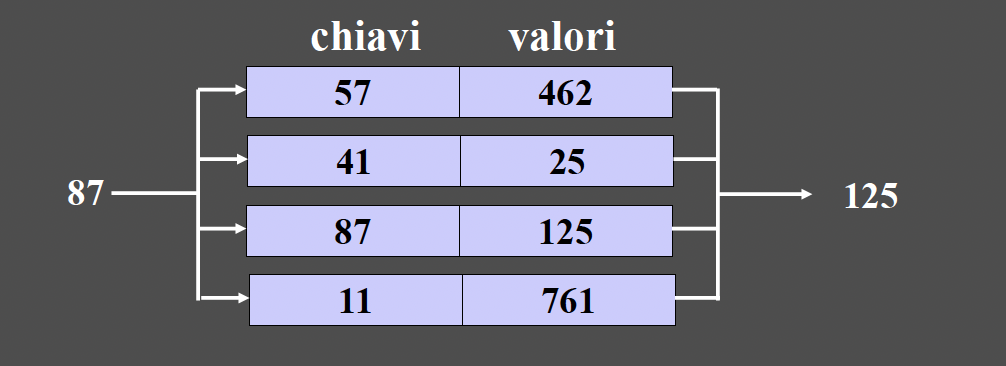
\includegraphics[width=0.50\linewidth]{images/chiave-valorePTB.png} \caption{chiave-valorePTB} \label{fig:9.9} \end{figure}

La TLB contiene una porzione della PT, costituita da coppie chiave–valore sotto forma di numero di pagina (chiave) e relativo frame (valore). Quando viene generato un indirizzo logico, il numero di pagina viene fornito alla TLB per ottenere il frame associato.

\cor{Hit Ratio nella TLB}{
    Il termine \emph{Hit Ratio} indica la percentuale di successi (hit) nella ricerca del numero di pagina nella TLB. Un maggiore hit ratio implica una minore degradazione delle prestazioni.
}

\ex{Calcolo delle prestazioni con e senza TLB}{
    Supponiamo: 1) un TLB perfetto, ossia accedere al TLB non costa tempo; 2) 10 nanosec per accedere alla RAM una volta tradotto l’indirizzo logico in fisico; 3) \emph{hit ratio} pari all'80\%. Il tempo medio di accesso in RAM sarà:
    
    \[
    10 \, \text{nsec} \times 0,80 + (10 + 10) \, \text{nsec} \times 0,20 = 12 \, \text{nsec}
    \]

    Il che comporta una degradazione delle prestazioni del 20\%.

    Se il TLB avesse invece un \emph{hit ratio} del 99\%, il tempo medio di accesso alla memoria sarebbe:

    \[
    10 \, \text{nsec} \times 0{,}99 + (10 + 10) \, \text{nsec} \times 0{,}01 = 10{,}1 \, \text{nsec}
    \]

    Questo porterebbe a una degradazione delle prestazioni di appena l'1\%.

    Se, invece, consideriamo che il TLB abbia un tempo di accesso maggiore di zero, diciamo all'incirca 1 nsec (cioè un decimo del tempo di accesso in RAM), con un \emph{hit ratio} del 99\% il tempo medio di accesso alla memoria sarebbe:

    \[
    (10 + 1) \, \text{nsec} \times 0{,}99 + (10 + 10) \, \text{nsec} \times 0{,}01 = 11{,}09 \, \text{nsec}
    \]

    In questo caso la degradazione delle prestazioni sarebbe di quasi l'11\%.

    Quando si verifica un \emph{miss} nella TLB, la coppia pagina-frame mancante viene recuperata attraverso la PT in RAM e copiata nella TLB. Questo permette che i successivi riferimenti alla stessa pagina usino la copia memorizzata nella TLB, riducendo il tempo di accesso.

    Se il TLB è pieno, una delle sue \emph{entry} deve essere sovrascritta, solitamente scegliendo l'elemento meno recentemente utilizzato (Least Recently Used, LRU) o selezionandone uno casuale.

    \nt{
    Al \emph{context switch} il TLB deve essere svuotato; verrà successivamente ripopolato con le coppie pagina-frame del nuovo processo in esecuzione.
    }

}

\subsection{Pagine condivise}
Quando due processi eseguono lo stesso codice, mantenere in memoria principale (MP) due copie identiche del codice non solo è inutile, ma spreca anche spazio in RAM. La paginazione facilita la condivisione del codice, poiché permette di memorizzare una sola copia di codice, condivisa tra i processi. Questo è possibile perché il codice, essendo \emph{non modificabile} durante l'esecuzione, viene definito come \emph{codice puro} o \emph{rientrante}.

\nt{
Una pagina condivisa può essere utilizzata per contenere codice di librerie dinamiche che diversi processi possono usare contemporaneamente, riducendo ulteriormente lo spazio richiesto in MP per il codice eseguito da più processi.
}

\begin{figure}[h] \centering 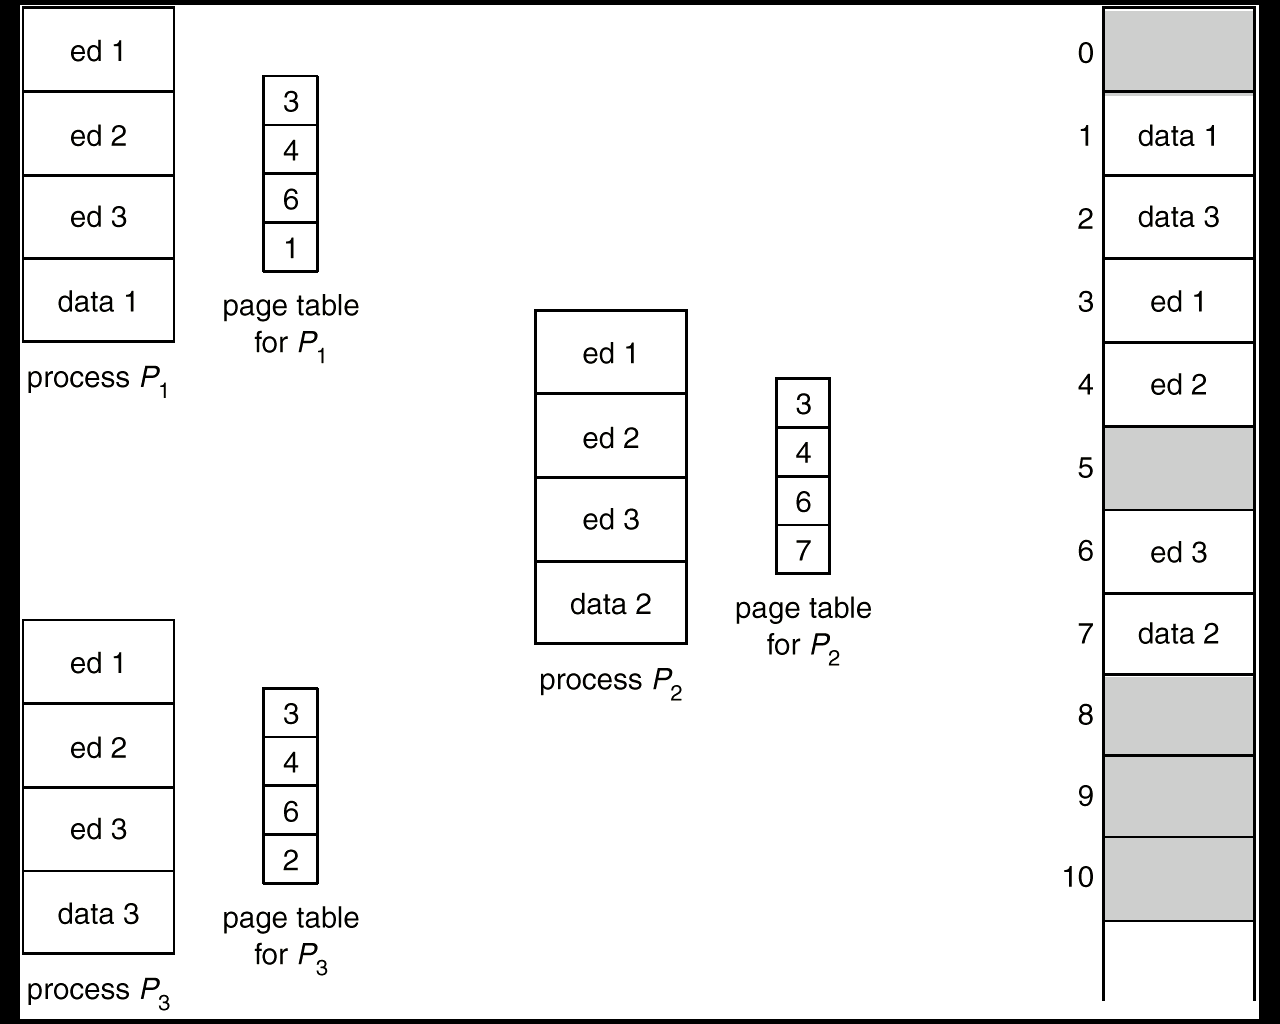
\includegraphics[width=0.45\linewidth]{images/shared_code_paginatedEnv.png} \caption{shared_code_paginatedEnv.png} \label{fig:9.9a} \end{figure}

\section{Paginazione a più livelli}

Nei moderni calcolatori, lo spazio di indirizzi logici può ormai raggiungere anche \(2^{64}\) byte. Per un sistema con \(2^{32}\) byte di spazio logico e pagine da 4 Kbyte (\(2^{12}\) byte), la \emph{Page Table} (PT) può avere fino a un milione (\(2^{20}\)) di entry. Se ogni entry occupa 4 byte, la PT del processo occuperà quindi 4 Mbyte, richiedendo ben 1024 frame per essere completamente contenuta in memoria principale (MP).

\qs{} {
Considerando questi numeri, è possibile ipotizzare la dimensione massima dello spazio di indirizzamento fisico del sistema?
}

Assumendo uno spazio logico di \(2^{32}\) byte, pagine da 4 Kbyte (\(2^{12}\) byte), e una dimensione di 4 byte per ogni entry della PT, si ha che ogni entry della PT deve contenere il numero di un frame del sistema. Con 32 bit a disposizione, possiamo numerare fino a \(2^{32}\) frame (dal frame 0 al frame \(2^{32}-1\)). Dunque, lo spazio di indirizzamento fisico del sistema può contenere al massimo \(2^{32}\) frame e avere una dimensione massima di \(2^{32} \times 2^{12} = 2^{44}\) byte.

\nt{
L'uso della paginazione consente di evitare la necessità di allocare grandi aree contigue di memoria principale, ma può succedere che la PT del processo attivo sia comunque molto grande, creando problemi di allocazione.
}

Una possibile soluzione consiste nell'implementare una \emph{paginazione a due livelli}, che suddivide la PT in pagine memorizzate in frame non adiacenti in MP. In questo caso, la PT vera e propria (ora chiamata \emph{PT interna}) richiede una \emph{PT esterna}, che indica in quali frame sono memorizzate le pagine della PT interna.

\ex{Esempio di paginazione a due livelli}{
Consideriamo una macchina con 32 bit di spazio di indirizzamento logico e fisico, e con pagine/frame da 4 Kbyte. In questo caso, un indirizzo logico sarà composto da:
\begin{itemize}
    \item 20 bit per il numero della pagina 
    \item 12 bit per l'offset all'interno della pagina.
\end{itemize}

Il numero di pagina \(p\), espresso su 20 bit, sarà quindi ulteriormente suddiviso in:
\begin{itemize}
    \item 10 bit più significativi (\(p_1\)): entry della PT esterna, che punta al frame \(F_1\) contenente una porzione della PT interna.
    \item 10 bit intermedi (\(p_2\)): offset nel frame \(F_1\).
\end{itemize}

Pertanto, l'indirizzo logico sarà strutturato come segue:

\[
\text{p} = \text{p}_1 \ \text{p}_2 \ \text{d}
\]
dove:
\begin{itemize}
    \item \(p_1\): 10 bit per la pagina esterna
    \item \(p_2\): 10 bit per la pagina interna
    \item \(d\): 12 bit per l'offset all'interno della pagina.
\end{itemize}
}
\begin{figure}[h] \centering 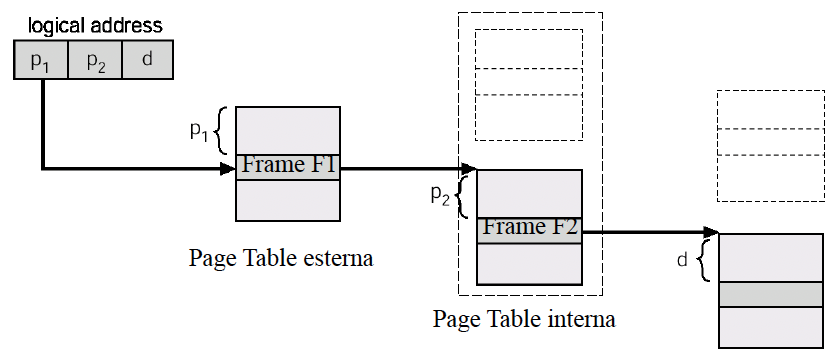
\includegraphics[width=0.50\linewidth]{images/traduzione_indirizzi_paginazione2Livelli.png} \caption{traduzione_indirizzi_paginazione2Livelli.png} \label{fig:9.16} \end{figure}

\ex{Esempio di calcolo dell'indirizzo fisico}{
Per comprendere il funzionamento della paginazione a due livelli in termini numerici, consideriamo un sistema in cui ogni entry delle PT occupa 4 byte (anche se tecnicamente sarebbero sufficienti 20 bit, poiché il numero massimo di frame è limitato). Prendiamo in esame la PT più grande, denominata \emph{PT interna}, che contiene \(2^{20}\) entry e quindi ha una dimensione di \(4 \times 2^{20}\) byte, richiedendo esattamente \(2^{10} = 1024\) frame.

La PT interna è quindi memorizzata in 1024 frame non contigui. Per tracciare la loro allocazione, il sistema operativo costruisce una \emph{PT esterna}, che occupa esattamente un frame (poiché ciascuna delle sue 1024 entry occupa 4 byte).

I passi per tradurre un indirizzo logico \(V\) di 32 bit in un indirizzo fisico sono i seguenti:
\begin{itemize}
    \item I 10 bit più significativi di \(V\), indicati come \(p_1\), servono per individuare una delle 1024 entry nella PT esterna, che funziona come un array di 1024 entry da 4 byte ciascuna.
    \item In questa entry, viene recuperato il numero del frame \(F_1\) che contiene una delle pagine della PT interna.
    \item Utilizzando i 10 bit intermedi di \(V\) (\(p_2\)), accediamo a una delle 1024 entry del frame \(F_1\). Questa entry contiene il numero del frame \(F_2\) che memorizza la pagina dell'indirizzo logico \(V\) (definito ora da \(p_1 p_2\)).
    \item Infine, aggiungendo l'offset \(d\) a \(F_2\), otteniamo l'indirizzo fisico finale.
\end{itemize}
}
\begin{figure}[h] \centering 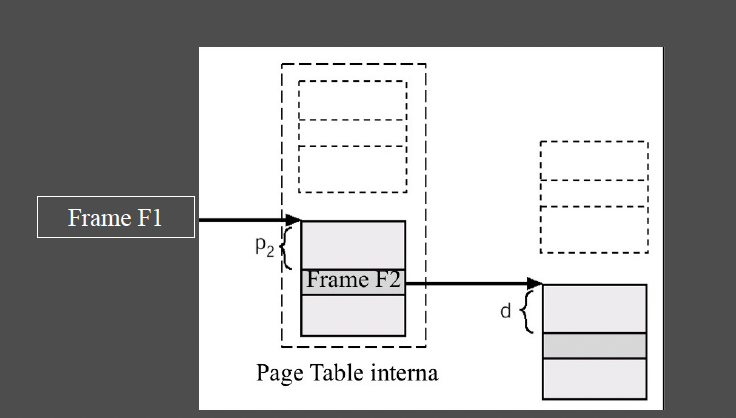
\includegraphics[width=0.50\linewidth]{images/ex_paginazione2Livelli.png} \caption{ex_paginazione2Livelli.png} \label{fig:9.17} \end{figure}


\section{Paginazione a due livelli}
La \textbf{paginazione a due livelli} è stata utilizzata, ad esempio, nei vecchi processori Pentium (lo vedremo successivamente come esempio pratico). Altre architetture, come la \textbf{VAX} di Digital Equipment Corporation (DEC), implementavano una \emph{PT esterna} composta da soli 4 elementi.

\qs{Gestione dello spazio logico su 64 bit}{
Che cosa accade con uno spazio di indirizzamento logico di 64 bit?\\
\textbf{Dimostrazione:} Con pagine da 4 Kbyte e 4 byte per entry nelle PT, la PT esterna può arrivare a occupare \(2^{44}\) byte. (Provate a verificare questo valore!)
}

Consideriamo ora la \textbf{PT interna} più grande con un indirizzamento logico a 64 bit:
\begin{itemize}
    \item Tale PT richiede \( \frac{2^{64}}{2^{12}} = 2^{52}\) entry, occupando dunque \(2^{52} \times 2^2 = 2^{54}\) byte.
    \item Questo corrisponde a \(\frac{2^{54}}{2^{12}} = 2^{42}\) frame.
    \item La PT esterna necessiterà quindi di \(2^{42}\) entry, ognuna da 4 byte, raggiungendo una dimensione di \(2^{42} \times 2^2 = 2^{44}\) byte.
\end{itemize}

\nt{
Con un indirizzamento logico a 64 bit, anche la PT esterna diventa così grande da necessitare una paginazione ulteriore. Questo problema non si limita alle architetture a 64 bit; anche alcune architetture a 32 bit implementavano paginazioni su più livelli:
}

\begin{itemize}
    \item \emph{SPARC} (SUN Microsystems) a 32 bit: utilizzava una paginazione a 3 livelli.
    \item CPU a 32 bit \emph{Motorola 68030}: implementava uno schema di paginazione a 4 livelli.
\end{itemize}

\clm{Overhead della paginazione su architetture a 64 bit}{}{
In sistemi a 64 bit, nemmeno 4 livelli di paginazione risultano sufficienti. Per esempio, l'architettura \emph{UltraSPARC} richiede fino a 7 livelli di paginazione. Se una pagina non è disponibile nel \emph{TLB}, la traduzione da indirizzo logico a fisico può richiedere l'attraversamento di 7 livelli di pagine in RAM, causando un notevole overhead.
}


\subsection{Page Table Invertita (IPT)}
Una soluzione alternativa adottata in alcune architetture a 64 bit è la \textbf{Tabella delle Pagine Invertita (IPT)}, la cui gestione presenta caratteristiche diverse rispetto alla paginazione tradizionale.

\begin{itemize}
    \item Una \emph{IPT} descrive l’occupazione dei frame nella memoria fisica. Al contrario delle \emph{PT}, esiste una sola \emph{IPT} per tutto il sistema (invece di una per ciascun processo), riducendo così lo spreco di memoria.
    \item La dimensione dell’\emph{IPT} dipende esclusivamente dalla dimensione della memoria primaria: ogni entry rappresenta un frame specifico, e il numero di entry totali equivale al numero di frame.
    \item L’indice di ogni entry dell’\emph{IPT} corrisponde al numero di un frame in memoria principale.
\end{itemize}

Ogni entry dell'\emph{IPT} è costituita da una coppia di valori:
\[
\langle \text{process-id}, \text{page-number} \rangle
\]
dove:
\begin{itemize}
    \item \emph{process-id} identifica il processo proprietario della pagina.
    \item \emph{page-number} indica il numero della pagina contenuta nel frame rappresentato da quella entry.
\end{itemize}

\begin{quote}
Ogni indirizzo logico generato dalla CPU è quindi una tripla:
\[
\langle \text{process-id}, \text{page-number}, \text{offset} \rangle
\]
Per generare l'indirizzo fisico, si cerca nella \emph{IPT} la coppia \(\langle \text{process-id}, \text{page-number} \rangle\). Se viene trovata nella \(i\)-esima entry, l'indirizzo fisico sarà \(\langle i, \text{offset} \rangle\).
\end{quote}

\clm{Vantaggi e svantaggi dell’IPT}{}{
Utilizzare una \emph{IPT} permette di risparmiare spazio, ma può aumentare il tempo di traduzione degli indirizzi logici in fisici, in quanto:
\begin{itemize}
    \item Per ottenere l’indirizzo fisico, è necessario scorrere la \emph{IPT} alla ricerca della entry contenente la coppia \(\langle \text{process-id}, \text{page-number} \rangle\), il che può richiedere centinaia o migliaia di accessi alla memoria principale (MP) se la \emph{IPT} è memorizzata in RAM.
    \item Tuttavia, l’uso di \emph{memorie associative} per contenere tutta o parte dell’\emph{IPT} consente la traduzione della maggior parte degli indirizzi senza un significativo impatto sulle prestazioni.
\end{itemize}
}

\section{Il supporto alla paginazione nei vecchi processori Intel}
La paginazione può, in teoria, essere implementata senza supporto hardware, ma un aiuto dall'hardware è fondamentale se si vogliono evitare significative degradazioni delle prestazioni. Oltre al supporto essenziale fornito dal \emph{Translation Lookaside Buffer (TLB)}, tutti i processori moderni offrono una gamma di facilitazioni per una gestione efficiente dei riferimenti in memoria.

Un esempio classico è rappresentato dalla famiglia dei vecchi processori Intel Pentium (ad esempio, Pentium 3 e 4). 

A scelta del sistema operativo che gira sul processore, è possibile utilizzare pagine da 4 Kbyte o da 4 Mbyte. Nel caso di pagine da 4 Kbyte, il processore adotta uno schema di paginazione a due livelli. La traduzione degli indirizzi da logici a fisici avviene nel modo consueto attraverso l'unità di paginazione:


\section{Conclusioni}
// TODO: :D